\documentclass{ximera}

\newcommand{\RR}{\mathbb R}
\renewcommand{\d}{\,d}
\newcommand{\dd}[2][]{\frac{d #1}{d #2}}
\renewcommand{\l}{\ell}
\newcommand{\ddx}{\frac{d}{dx}}
\newcommand{\dfn}{\textbf}
\newcommand{\eval}[1]{\bigg[ #1 \bigg]}


\title[Dig-In:]{Quadric surfaces}

\outcome{Define a quadric surface.}
\outcome{Identify basic quadric surfaces.}
\outcome{Use sections to identify surfaces.}
\outcome{Use the second derivative test to identify quadric surfaces.}

\begin{document}
\begin{abstract}
  We will get to know some basic quadric surfaces.
\end{abstract}
\maketitle

As we have seen, if we look at the set of points that satisfy an
equation
\[
F(x,y,z)=0
\]
where $F:\R^3\to\R$, we obtain a surface in $\R^3$. A basic class of
surfaces are the \textit{quadric surfaces}.

\begin{definition}
A \dfn{quadric surface} in $\R^3$ is a surface of the form
\[
Ax^2 + By^2 + Cz^2 + Dxy + Exz+ Fyz + Gx + Hy + I z + J = 0
\]
where $A$, $B$, $C$, $D$, $E$, $F$, $G$, $H$, $I$, and $J$ are
constants and at least one of $A$, $B$, $C$, $D$, $E$, or $F$ are
nonzero.
\end{definition}

\begin{question}
  Which of the following are quadric surfaces?
  \begin{selectAll}
    \choice[correct]{$x^2 = 0$}
    \choice{$y=0$}
    \choice[correct]{$z=y^2$}
  \end{selectAll}
\end{question}

\begin{warning}
  Do not confuse a \textit{quadric} with a quadratic, or quartic, as
  these are different beasts entirely.
\end{warning}

We will be interested in a special class of quadric surfaces, those
that arise naturally when computing the Taylor polynomial of a surface
$z=F(x,y)$ at a point $\vec{c}$ where:
\[
F^{(1,0)}(\vec{c}) = 0 = F^{(0,1)}(\vec{c})
\]
In this case, the quadric is of the form:
\begin{align*}
  z = &F^{(2,0)}(\vec{c})(x-c_1)^2 \\
  &+ F^{(0,2)}(\vec{c})(y-c_2)^2 \\
  &+ F^{(1,1)}(\vec{c}) (x-c_1)(y-c_2)\\
  &+ F(\vec{c})
\end{align*}
Why are we doing this?
\begin{quote}
  \textbf{Understanding quadric surfaces will help us find extrema of
    surfaces.}
\end{quote}

In what follows, we will study each shape by considering various
\textit{sections} of the surface.

\begin{definition}
  A \dfn{section} of a surface is the intersections of a surface with
  a plane.
\end{definition}

\begin{question}
  Consider the following surface:
  \[
  z = 6x^2 + y^2 + 5 xy
  \]
  Compute the section of the surface given by the plane $y=0$.
  \begin{prompt}
    \[
    z = \answer{6x^2}
    \]
  \end{prompt}
  \begin{question}
    Does this parabola open ``up'' or ``down?''
    \begin{prompt}
    \begin{multipleChoice}
      \choice[correct]{up}
      \choice{down}
    \end{multipleChoice}
    \end{prompt}
    \begin{question}
      Compute the section of the surface given by the plane $y=-2.5 x$.
      \begin{prompt}
        \[
        z = \answer{6x^2 + 6.25 x^2 - 12.5x^2}
        \]
      \end{prompt}
      \begin{question}
        Does this parabola open ``up'' or ``down?''
        \begin{prompt}
          \begin{multipleChoice}
            \choice{up}
            \choice[correct]{down}
          \end{multipleChoice}
        \end{prompt}
      \end{question}
    \end{question}
  \end{question}
\end{question}

  





\section{Elliptic paraboloids}

An \dfn{elliptic paraboloid} is a surface with graph:
\begin{image}
  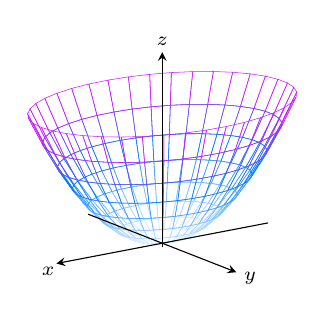
\begin{tikzpicture}
    \begin{axis}%
      [width=175pt,tick label style={font=\scriptsize},axis on top,
	axis lines=center,
	view={145}{20},
	name=myplot,
	xtick=\empty,
	ytick=\empty,
	ztick=\empty,
	ymin=-2.5,ymax=2.5,
	xmin=-3.5,xmax=3.5,
	zmin=-.1, zmax=5.5,
	every axis x label/.style={at={(axis cs:\pgfkeysvalueof{/pgfplots/xmax},0,0)},xshift=-3pt,yshift=-3pt},
	xlabel={\scriptsize $x$},
	every axis y label/.style={at={(axis cs:0,\pgfkeysvalueof{/pgfplots/ymax},0)},xshift=5pt,yshift=-2pt},
	ylabel={\scriptsize $y$},
	every axis z label/.style={at={(axis cs:0,0,\pgfkeysvalueof{/pgfplots/zmax})},xshift=0pt,yshift=4pt},
	zlabel={\scriptsize $z$},
        colormap/cool
      ]
      
      \addplot3[domain=0:360,y domain=0:2,color=black!40,mesh,samples=40,samples y=10,very thin,z buffer=sort] ({2*cos(x)*y},{sin(x)*y},{y^2});
    \end{axis}
  \end{tikzpicture}
\end{image}
and equation, after moving the vertex to the origin:
\[
z=\pm\frac{x^2}{a^2}\pm\frac{y^2}{b^2}
\]
To understand this surface better consider the sections when:
\begin{itemize}
  \item $x=d$, in this case we now have $z = \pm\frac{d^2}{a^2} \pm
    \frac{y^2}{b^2}$, a parabola.
  \item $y=d$, in this case we now have $z = \pm\frac{x^2}{a^2} \pm
    \frac{d^2}{b^2}$, a parabola.
  \item $z=d$, in this case we now have $d = \pm\frac{x^2}{a^2} \pm
    \frac{y^2}{b^2}$, an ellipse.
\end{itemize}
\begin{image}
  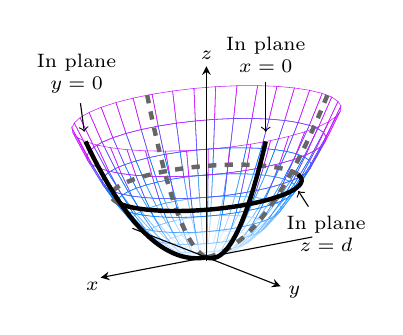
\begin{tikzpicture}
    \begin{axis}%
      [width=175pt,tick label style={font=\scriptsize},axis on top,
	axis lines=center,
        clip=false,
	view={145}{20},
	name=myplot,
	xtick=\empty,
	ytick=\empty,
	ztick=\empty,
	ymin=-2.5,ymax=2.5,
	xmin=-3.5,xmax=3.5,
	zmin=-.1, zmax=5.5,
	every axis x label/.style={at={(axis cs:\pgfkeysvalueof{/pgfplots/xmax},0,0)},xshift=-3pt,yshift=-3pt},
	xlabel={\scriptsize $x$},
	every axis y label/.style={at={(axis cs:0,\pgfkeysvalueof{/pgfplots/ymax},0)},xshift=5pt,yshift=-2pt},
	ylabel={\scriptsize $y$},
	every axis z label/.style={at={(axis cs:0,0,\pgfkeysvalueof{/pgfplots/zmax})},xshift=0pt,yshift=4pt},
	zlabel={\scriptsize $z$},colormap/cool
      ]
      
      \addplot3[domain=0:360,y domain=0:2,mesh,samples=40,samples y=10,very thin,z buffer=sort] ({2*cos(x)*y},{sin(x)*y},{y^2});
      
      \addplot3[domain=170:360,dashed,ultra thick,smooth,samples y=0,black!60,%surf,%fill=white,
        samples=30,] ({2*cos(x)*sqrt(2)},{sin(x)*sqrt(2)},{2});

      \addplot3[domain=-2:0,dashed,ultra thick,smooth,samples y=0,black!60,%surf,%fill=white,
        samples=30,] ({2*x},{0},{x^2});

      \addplot3[domain=-2:0,dashed,ultra thick,smooth,samples y=0,black!60,%surf,%fill=white,
        samples=30,] ({0},{x},{x^2});
      
      \addplot3[domain=0:170,ultra thick,smooth,samples y=0,black,%surf,%fill=white,
        samples=30,] ({2*cos(x)*sqrt(2)},{sin(x)*sqrt(2)},{2});
      
      \addplot3[domain=0:2,ultra thick,smooth,samples y=0,black,%surf,%fill=white,
        samples=30,] ({2*x},{0},{x^2});

      \addplot3[domain=0:2,ultra thick,smooth,samples y=0,black,%surf,%fill=white,
          samples=30,] ({0},{x},{x^2});
      
        \draw (axis cs:4.3,0,6) node[align=center] (A1) {\scriptsize In plane\\[-4pt] \scriptsize $y=0$};
        \draw (axis cs:4,0,4) node (A2) {};
        \draw [->](A1)--(A2);
        
        \draw (axis cs:0,2,6.5) node[align=center] (B1) {\scriptsize In plane\\[-4pt] \scriptsize $x=0$};
        \draw (axis cs:0,2,4) node (B2) {};
        \draw [->](B1)--(B2);

        \draw (axis cs:-2,2,1) node[align=center] (C1) {\scriptsize In plane\\[-4pt] \scriptsize $z=d$};
        \draw (axis cs:-2.83,0,2) node [below] (C2) {};
        \draw [->](C1)--(C2);
        %\foreach \z in {-6.28,-4.71,-1.57,1.57,6.28}
        %{\addplot3[domain=-2:2,,thick,smooth,samples y=0,{\colortwo},%surf,%fill=white,
        %samples=30,] ({sin(deg(\z))},{x},{\z});
        %}
    \end{axis}
  \end{tikzpicture}
\end{image}
\[
\begin{array}{cc}
\textbf{Plane} & \textbf{Section} \\ \hline
x=d  & \text{Parabola} \\
y=d  & \text{Parabola}\\
z=d  & \text{Ellipse}
\end{array}
\]




\section{Hyperbolic paraboloids}

A \dfn{hyperbolic paraboloid} is a surface with graph:
\begin{image}
  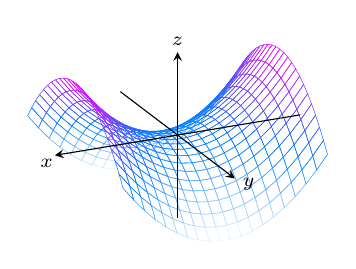
\begin{tikzpicture}
    \begin{axis}%
      [width=175pt,tick label style={font=\scriptsize},axis on top,
	axis lines=center,
	view={155}{30},
	name=myplot,
	xtick=\empty,
	ytick=\empty,
	ztick=\empty,
	ymin=-1.2,ymax=1.2,
	xmin=-1.2,xmax=1.2,
	zmin=-1.2, zmax=1.2,
	every axis x label/.style={at={(axis cs:\pgfkeysvalueof{/pgfplots/xmax},0,0)},xshift=-3pt,yshift=-3pt},
	xlabel={\scriptsize $x$},
	every axis y label/.style={at={(axis cs:0,\pgfkeysvalueof{/pgfplots/ymax},0)},xshift=5pt,yshift=-2pt},
	ylabel={\scriptsize $y$},
	every axis z label/.style={at={(axis cs:0,0,\pgfkeysvalueof{/pgfplots/zmax})},xshift=0pt,yshift=4pt},
	zlabel={\scriptsize $z$},
        colormap/cool
      ]

      \addplot3[domain=-1:1,smooth,y domain=-1:1,mesh,samples=20,samples y=25,very thin,z buffer=sort] ({x},{y},{x^2-y^2});
    \end{axis}
  \end{tikzpicture}
\end{image}
and equation, after moving the vertex to the origin:
\[
z=\pm\frac{x^2}{a^2}\mp\frac{y^2}{b^2}
\]
To understand this surface better consider the sections when:
\begin{itemize}
  \item $x=d$, in this case we now have $z = \pm\frac{d^2}{a^2} \mp
    \frac{y^2}{b^2}$, a parabola.
  \item $y=d$, in this case we now have $z = \pm\frac{x^2}{a^2} \mp
    \frac{d^2}{b^2}$, a parabola that opens the \textit{opposite}
    direction as the previous one.
  \item $z=d$, in this case we now have $d = \pm\frac{x^2}{a^2} \mp
    \frac{y^2}{b^2}$, a hyperbola.
\end{itemize}
\begin{image}
  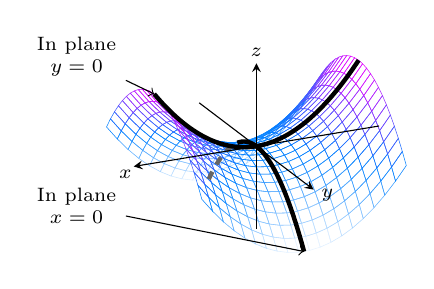
\begin{tikzpicture}
    \begin{axis}%
      [width=175pt,tick label style={font=\scriptsize},axis on top,
	axis lines=center,
	view={155}{30},
	name=myplot,
	xtick=\empty,
	ytick=\empty,
	ztick=\empty,
	ymin=-1.2,ymax=1.2,
	xmin=-1.2,xmax=1.2,
	zmin=-1.2, zmax=1.2,
	every axis x label/.style={at={(axis cs:\pgfkeysvalueof{/pgfplots/xmax},0,0)},xshift=-3pt,yshift=-3pt},
	xlabel={\scriptsize $x$},
	every axis y label/.style={at={(axis cs:0,\pgfkeysvalueof{/pgfplots/ymax},0)},xshift=5pt,yshift=-2pt},
	ylabel={\scriptsize $y$},
	every axis z label/.style={at={(axis cs:0,0,\pgfkeysvalueof{/pgfplots/zmax})},xshift=0pt,yshift=4pt},
	zlabel={\scriptsize $z$},colormap/cool
      ]
      
      \addplot3[domain=-1:1,smooth,y domain=-1:1,mesh,samples=20,samples y=25,very thin,z buffer=sort] ({x},{y},{x^2-y^2});

      \addplot3[domain=-1:-.4,dashed,ultra thick,smooth,samples y=0,black!60,%surf,%fill=white,
        samples=30,] ({0},{x},{-x^2});
      
      \addplot3[domain=-1:1,ultra thick,smooth,samples y=0,black,%surf,%fill=white,
        samples=30,] ({x},{0},{x^2});
      
      \addplot3[domain=-.4:1,ultra thick,smooth,samples y=0,black,%surf,%fill=white,
        samples=30,] ({0},{x},{-x^2});
      
      
      \draw (axis cs:1.,0,1) node (A2) {};
      \draw (axis cs:0,1,-1) node (B2) {};
      %\draw (axis cs:0,1.5,0.3) node (C2) {};
      
    \end{axis}
    
    \draw (0,3) node [align=center](A1) {\scriptsize In plane\\[-4pt] \scriptsize $y=0$};
    \draw (0,1.1) node [align=center](B1) {\scriptsize In plane\\[-4pt] \scriptsize $x=0$};
    %
    \draw [->](A1)--(A2.center);
    \draw [->](B1)--(B2.center);
    %\draw [->](C1)--(C2.center);
  \end{tikzpicture}
\end{image}
We'll give an additional graph to show the hyperbolas:
\begin{image}
  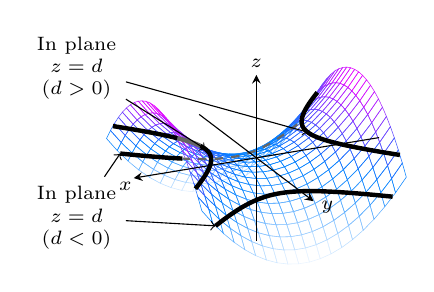
\begin{tikzpicture}
    \begin{axis}%
      [width=175pt,tick label style={font=\scriptsize},axis on top,
        axis lines=center,
        view={155}{30},
        name=myplot,
        xtick=\empty,
        ytick=\empty,
        ztick=\empty,
        ymin=-1.2,ymax=1.2,
        xmin=-1.2,xmax=1.2,
        zmin=-1.2, zmax=1.2,
        every axis x label/.style={at={(axis cs:\pgfkeysvalueof{/pgfplots/xmax},0,0)},xshift=-3pt,yshift=-3pt},
        xlabel={\scriptsize $x$},
        every axis y label/.style={at={(axis cs:0,\pgfkeysvalueof{/pgfplots/ymax},0)},xshift=5pt,yshift=-2pt},
        ylabel={\scriptsize $y$},
        every axis z label/.style={at={(axis cs:0,0,\pgfkeysvalueof{/pgfplots/zmax})},xshift=0pt,yshift=4pt},
        zlabel={\scriptsize $z$},
        colormap/cool
      ]
      
  \addplot3[domain=-1:1,y domain=-1:1,mesh,samples=20,samples y=25,very thin,z buffer=sort] ({x},{y},{x^2-y^2});
  
  \addplot3[domain=-10:60,ultra thick,smooth,samples y=0,black,%surf,%fill=white,
    samples=30,] ({.5*sec(x)},{.5*tan(x)},{.25});
  \addplot3[domain=-35:-10,ultra thick,smooth,samples y=0,black!60,%surf,%fill=white,
    samples=30,] ({.5*sec(x)},{.5*tan(x)},{.25});
  \addplot3[domain=-60:-35,ultra thick,smooth,samples y=0,black,%surf,%fill=white,
    samples=30,] ({.5*sec(x)},{.5*tan(x)},{.25});
  
  \addplot3[domain=-60:60,ultra thick,smooth,samples y=0,black,%surf,%fill=white,
    samples=30,] ({-.5*sec(x)},{.5*tan(x)},{.25});
  
  
  \addplot3[domain=-60:60,ultra thick,smooth,samples y=0,black,%surf,%fill=white,
    samples=30,] ({.5*tan(x)},{.5*sec(x)},{-.25});
  \addplot3[domain=40:60,ultra thick,smooth,samples y=0,black,%surf,%fill=white,
    samples=30,] ({.5*tan(x)},{-.5*sec(x)},{-.25});
  \addplot3[domain=-60:40,dashed,thick,smooth,samples y=0,black!60,%surf,%fill=white,
    samples=30,] ({.5*tan(x)},{-.5*sec(x)},{-.25});

  \draw (axis cs:.5,0,.25) node (A2) {};
  \draw (axis cs:-.5,0,.25) node (A3) {};
  \draw (axis cs:.866,1,-.25) node (B2) {};
  \draw (axis cs:.866,-1,-.25) node (B3) {};
  %\draw (axis cs:0,1.5,0.3) node (C2) {};
\end{axis}
\draw (0,3) node [align=center](A1) {\scriptsize In plane\\[-4pt] \scriptsize $z=d$\\[-4pt] \scriptsize $(d>0)$};
\draw (0,1.1) node [align=center](B1) {\scriptsize In plane\\[-4pt] \scriptsize $z=d$\\[-4pt] \scriptsize $(d<0)$};
%\draw (4.6,2) node [align=center](C1) {\scriptsize in plane\\[-4pt] \scriptsize $z=0$};

\draw [->](A1)--(A2.center);
\draw [->](A1)--(A3.center);
\draw [->](B1)--(B2.center);
\draw [->](B1)--(B3.center);
%\draw [->](C1)--(C2.center);
  \end{tikzpicture}
\end{image}
\[
\begin{array}{cc}
\textbf{Plane}  & \textbf{Section} \\ \hline
x=d & \text{Parabola}\\
y=d & \text{Parabola}\\
z=d & \text{Hyperbola}
\end{array}
\]

\section{Identifying quadric surfaces}

Let's start by working a specific example.

\begin{example}
  Consider the surface:
  \[
  z = x^2+4y^2-5xy
  \]
  Is this surface an elliptic paraboloid or a hyperbolic paraboloid?
  \begin{explanation}
    We'll work somewhat naively. Consider the plane $y= mx$. This
    plane is perpendicular to the $(x,y)$-plane. If we intersect this
    plane with the surface above, we will find a parabola. If we can
    change the direction that the parabola opens by varying $m$, then
    our surface is a hyperbolic paraboloid. If we cannot change the
    direction that the parabola opens by varying $m$, then our surface
    is an elliptic paraboloid. Start by setting $m = 0$. In this case
    we find:
    \[
    z = \answer[given]{x^2}
    \]
    This is a parabola that opens ``up'' in the $(x,z)$-plane. Can we
    find a parabola that opens ``down'' by varying $m$? Intersecting
    the surface $z = x^2 + 4y^2 -5xy$ and $y=mx$ we find:
    \begin{align*}
      z &= \answer[given]{x^2 + 4 m^2 x^2 -5 x^2 m}\\
      &=x^2\left(\answer[given]{4 m^2-5m + 1}\right)
    \end{align*}
    This parabola will open ``downward'' when we can find $m$ such
    that $4 m^2-5m + 1$ is negative. The expression $4 m^2-5m + 1$ is zero when
    \begin{align*}
      m &= 1/4\\
      m &= \answer[given]{1}.
    \end{align*}
    Let's draw a sign-chart:
    \begin{image}
      \begin{tikzpicture}
	\begin{axis}[
            trim axis left,
            scale only axis,
            domain=0:1.75,
            ymax=2,
            ymin=-2,
            axis lines=none,
            height=3cm, %% Hard coded height! 
            width=\textwidth, %% width
          ]
          \addplot [draw=none, fill=fill1, domain=(0:1/4)] {2} \closedcycle;
          \addplot [draw=none, fill=fill2, domain=(1/4:1)] {2} \closedcycle;
          \addplot [draw=none, fill=fill1, domain=(1:1.75)] {2} \closedcycle;
                    
          \addplot [->,textColor] plot coordinates {(0,0) (1.75,0)}; %% axis{0};
          
          \addplot [dashed, textColor] plot coordinates {(1/4,0) (1/4,2)};
          \addplot [dashed, textColor] plot coordinates {(1,0) (1,2)};
                    
          \node at (axis cs:1/4,0) [anchor=north,textColor] {\footnotesize$1/4$};
          \node at (axis cs:1,0) [anchor=north,textColor] {\footnotesize$1$};

          \node at (axis cs:.125,1) [textColor] {\footnotesize$+$};
          \node at (axis cs:.625,1) [textColor] {\footnotesize$-$};
          \node at (axis cs:1.375,1) [textColor] {\footnotesize$+$};
          

        \end{axis}
      \end{tikzpicture}
    \end{image}
    Since the intersection of $z=x^2+4y^2-5xy$ with the plane $y=0$ is
    a parabola that opens ``up'' in the $(x,z)$-plane, and the
    intersection of the surface with the plane $y = x/2$ (or $y=mx$
    where $m$ is between $1/4$ and $1$) is a parabola that opens
    ``down'' in the $(x,z)$-plane, we have a hyperbolic paraboloid.
    \begin{onlineOnly}
      For your viewing pleasure, we've included a graph of the
      hyperbolic paraboloid and the plane:
      \begin{center}    
        \geogebra{QZdktQMQ}{800}{600}
      \end{center}
    \end{onlineOnly}
  \end{explanation}
\end{example}

Later in this course, we will be looking at quadric surfaces of the
form
\begin{align*}
  z = &\left(\frac{1}{2}\right)F^{(2,0)}(\vec{c})(x-c_1)^2\\
  &+ \left(\frac{1}{2}\right)F^{(0,2)}(\vec{c})(y-c_2)^2 \\
  &+ F^{(1,1)}(\vec{c}) (x-c_1)(y-c_2)\\
  &+ F(\vec{c}).
\end{align*}
and trying to identify them as either elliptic paraboloids, or as
hyperbolic paraboloids. In what follows, let
\[
\sign(x) =
\begin{cases}
  1  &\text{if $x>0$,}\\
  -1 &\text{if $x<0$,}\\
  0  &\text{if $x=0$.}
\end{cases}
\]
This will aid in our analysis of the quadric surfaces.

\subsection{The pure partials have opposite signs}
If
\[
\sign(F^{(2,0)}(\vec{c})) = -\sign(F^{(0,2)}(\vec{c})),
\]
then we can examine the following sections:
\[
y= c_2 \quad\text{and}\quad x = c_1
\]
If $y=c_2$ then the surface
\begin{align*}
  z = &\left(\frac{1}{2}\right)F^{(2,0)}(\vec{c})(x-c_1)^2\\
  &+ \left(\frac{1}{2}\right)F^{(0,2)}(\vec{c})(y-c_2)^2 \\
  &+ F^{(1,1)}(\vec{c}) (x-c_1)(y-c_2)\\
  &+ F(\vec{c}).
\end{align*}
becomes
\[
z = \left(\frac{1}{2}\right)F^{(2,0)}(\vec{c})(x-c_1)^2 + F(\vec{c}),
\]
and this is a parabola that opens in the $z$-direction of the sign of
$F^{(2,0)}(\vec{c})$.

If $x=c_1$ then the surface becomes
\[
z = \left(\frac{1}{2}\right)F^{(0,2)}(\vec{c})(y-c_2)^2 + F(\vec{c}),
\]
and this is a parabola that opens in the $z$-direction of the sign of
$F^{(0,2)}(\vec{c})$. Since 
\[
\sign(F^{(2,0)}(\vec{c})) = -\sign(F^{(0,2)}(\vec{c})),
\]
we see that when the pure partials have opposite signs, then the
quadric surface is a hyperbolic paraboloid.

\subsection{The pure partials have the same sign}
If 
\[
\sign(F^{(2,0)}(\vec{c})) = \sign(F^{(0,2)}(\vec{c})),
\]
then we start by examining the section:
\[
y -c_2 = m (x-c_1)
\]
Substituting this into the surface above, we find
\begin{align*}
  z = &\left(\frac{1}{2}\right)F^{(2,0)}(\vec{c})(x-c_1)^2\\
  &+ m^2 \left(\frac{1}{2}\right)F^{(0,2)}(\vec{c})(x-c_1)^2\\
  &+ m F^{(1,1)}(\vec{c}) (x-c_1)^2 \\
  &+ F(\vec{c}).
\end{align*}
Factoring and rearranging, set
\[
A = m^2 \left(\frac{1}{2}\right)F^{(0,2)}(\vec{c}) + m F^{(1,1)}(\vec{c}) + \left(\frac{1}{2}\right)F^{(2,0)}(\vec{c})
\]
and now 
\begin{align*}
z = (x-c_1)^2 A + F(\vec{c}).
\end{align*}
This is a parabola that opens in the $z$-direction of the sign of
$F^{(2,0)}(\vec{c})$ when
\[
A = m^2 \left(\frac{1}{2}\right)F^{(0,2)}(\vec{c}) + m F^{(1,1)}(\vec{c}) + \left(\frac{1}{2}\right)F^{(2,0)}(\vec{c})
\]
has the same sign as $F^{(2,0)}(\vec{c})$.  The parabola opens in the
opposite direction, when
\[
A = m^2 \left(\frac{1}{2}\right)F^{(0,2)}(\vec{c}) + m F^{(1,1)}(\vec{c}) + \left(\frac{1}{2}\right)F^{(2,0)}(\vec{c})
\]
has the opposite sign as $F^{(2,0)}(\vec{c})$.  We can find a $m$ that
produces this opposite sign when the quadratic equation, in the
variable $m$,
\[
m^2 \left(\frac{1}{2}\right)F^{(0,2)}(\vec{c}) + m F^{(1,1)}(\vec{c}) + \left(\frac{1}{2}\right)F^{(2,0)}(\vec{c}) = 0
\]
has two real solutions. Let's investigate using the quadratic formula:
\[
m = \frac{- F^{(1,1)}\pm(\vec{c})\sqrt{F^{(1,1)}(\vec{c})^2-F^{(2,0)}(\vec{c})F^{(0,2)}(\vec{c})}}{F^{(0,2)}(\vec{c})}
\]
We see that there are two real solutions for $m$ when
\[
F^{(1,1)}(\vec{c})^2-F^{(2,0)}(\vec{c})F^{(0,2)}(\vec{c})>0
\]
or equivalently when
\[
F^{(2,0)}(\vec{c})F^{(0,2)}(\vec{c})-F^{(1,1)}(\vec{c})^2<0.
\]
So, we see that when the pure partials have the same sign, the quadric
surface is a hyperbolic paraboloid when
\[
F^{(2,0)}(\vec{c})F^{(0,2)}(\vec{c})-F^{(1,1)}(\vec{c})^2<0,
\]
and an elliptic paraboloid when 
\[
F^{(2,0)}(\vec{c})F^{(0,2)}(\vec{c})-F^{(1,1)}(\vec{c})^2>0.
\]

\section{The second derivative test}

Given a function $F:\R^2\to \R$, and a point $\vec{c}$ where
\[
F^{(1,0)}(\vec{c}) = 0 = F^{(0,1)}(\vec{c}),
\]
our work above allows us to identify what a surface looks like
locally. Specifically we get what is known as the second derivative test:

\begin{theorem}[Second derivative test]
  Given a function $F:\R^2\to \R$, and a point $\vec{c}$ where
  \[
  F^{(1,0)}(\vec{c}) = 0 = F^{(0,1)}(\vec{c}) 
  \]
  set
  \[
  D(\vec{c}) = F^{(2,0)}(\vec{c})F^{(0,2)}(\vec{c})-F^{(1,1)}(\vec{c})^2.
  \]
  \begin{itemize}
  \item If $D(\vec{c})>0$, then $F$ locally looks like an elliptic paraboloid.
  \item	If $D(\vec{c})<0$, then $F$ locally looks like a hyperbolic paraboloid.
  \item If $D(\vec{c})=0$, the test is inconclusive.
  \end{itemize}
\end{theorem}

Try your hand at identifying local behavior of a surface.


\begin{question}
  Consider $F(x,y) = x^3-3x-y^2+4y$. Does this surface locally look like
  an elliptic paraboloid or a hyperbolic paraboloid at the point
  $(-1,2)$?
  \begin{prompt}
    Compute:
    \begin{align*}
      \pp[F]{x} &= \answer{3x^2-3}\\
      \pp[F]{y} &= \answer{4-2y}\\
      \frac{\partial^2F}{\partial x^2} &= \answer{6x}\\
      \frac{\partial^2F}{\partial y^2} &= \answer{-2}\\
      \frac{\partial^2F}{\partial x\partial y} &= \answer{0}\\
    \end{align*}
    \begin{question}
      \[
      D(-1,2) = \answer{12}
      \]
      \begin{question}
        \begin{multipleChoice}
          \choice[correct]{An elliptic paraboloid.}
          \choice{A hyperbolic paraboloid.}
          \choice{We cannot tell.}
        \end{multipleChoice}
      \end{question}
    \end{question}
  \end{prompt}
  \begin{question}
  Again consider $F(x,y) = x^3-3x-y^2+4y$. Does this surface locally look like
  an elliptic paraboloid or a hyperbolic paraboloid at the point
  $(1,2)$?
  \begin{prompt}
    Compute:
    \[
    D(-1,2) = \answer{-12}
    \]
    \begin{question}
      \begin{multipleChoice}
        \choice{An elliptic paraboloid.}
        \choice[correct]{A hyperbolic paraboloid.}
        \choice{We cannot tell.}
      \end{multipleChoice}
    \end{question}
  \end{prompt}
  \end{question}
\end{question}




\begin{question}
  Consider $F(x,y) = e^{x^2+y^2}$. Does this surface locally look like
  an elliptic paraboloid or a hyperbolic paraboloid at the point
  $(0,0)$?
  \begin{prompt}
    Compute:
    \begin{align*}
      \pp[F]{x} &= \answer{2x e^{x^2+y^2}}\\
      \pp[F]{y} &= \answer{2y e^{x^2+y^2}}\\
      \frac{\partial^2F}{\partial x^2} &= \answer{2 e^{x^2+y^2}+4x^2 e^{x^2+y^2}}\\
      \frac{\partial^2F}{\partial y^2} &= \answer{2 e^{x^2+y^2}+4y^2 e^{x^2+y^2}}\\
      \frac{\partial^2F}{\partial x\partial y} &= \answer{4 x y e^{x^2+y^2}}\\
    \end{align*}
    \begin{question}
      \[
      D(0,0) = \answer{4}
      \]
      \begin{question}
        \begin{multipleChoice}
          \choice[correct]{An elliptic paraboloid.}
          \choice{A hyperbolic paraboloid.}
          \choice{We cannot tell.}
        \end{multipleChoice}
      \end{question}
    \end{question}
  \end{prompt}
\end{question}

\begin{question}
  Consider $F(x,y) = x y e^{-xy}$. Does this surface locally look like
  an elliptic paraboloid or a hyperbolic paraboloid at the point
  $(0,0)$?
  \begin{prompt}
    Compute:
    \begin{align*}
      \pp[F]{x} &= \answer{y e^{-x y}-xy^2e^{-x y}}\\
      \pp[F]{y} &= \answer{x e^{-x y}-x^2ye^{-x y}}\\
      \frac{\partial^2F}{\partial x^2} &= \answer{xy^3e^{-xy}-2y^2e^{-xy}}\\
      \frac{\partial^2F}{\partial y^2} &= \answer{x^3ye^{-xy}-2x^2e^{-xy}}\\
      \frac{\partial^2F}{\partial x\partial y} &= \answer{x^2 y^2 e^{-x y}-3 x y e^{-x y}+e^{-x y}}\\
    \end{align*}
    \begin{question}
      \[
      D(0,0) = \answer{-1}
      \]
      \begin{question}
        \begin{multipleChoice}
          \choice{An elliptic paraboloid.}
          \choice[correct]{A hyperbolic paraboloid.}
          \choice{We cannot tell.}
        \end{multipleChoice}
      \end{question}
    \end{question}
  \end{prompt}
\end{question}





\end{document}

